\section{Theorie}
\label{sec:Theorie}

\subsection{Konkave und konvexe Linsen, Konstruktion von Strahlengängen und Linsenfehler}

In Abbildung \ref{fig:konvex_duenn} sind einmal gesammelt (fast) alle Abkürzungen zu sehen, die im Folgenden gehäuft auftreten. 
\begin{figure}
    \centering
    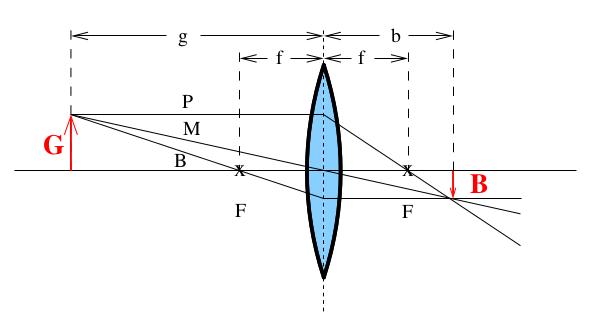
\includegraphics[width=0.75\textwidth]{plots/Linse1.png}
    \caption{Eine dünne konvexe Linse zur Veranschaulichung der geometrischen Bedeutung der im Folgenden verwendeten Begriffe\cite{Versuchsanleitung}.}
    \label{fig:konvex_duenn}
\end{figure}
$G$ gibt die Größe des Gegenstands an, von dem Licht auf die entsprechende Linse fällt, $B$ ist die Größe des entstehenden, 
scharf gestellten Bildes. Die Größen werden jeweils immer bis zur optischen Achse (horizontale Linie in der Abbildung) gemessen. 
Vom Gegenstand ausgehend können drei Strahlen eingezeichnet werden, um das Bild der Lichtstrahlen nach Kontakt mit der Linse 
zu konstruieren: Der Parallelstrahl $P$ geht parallel zur optischen Achse von der Spitze des Gegenstands zur Linse und wird nach Brechung zu einem 
Brennpunktstrahl $B$, da er durch den hinter der Linse befindlichen Brennpunkt $F$ geht. 
Analog dazu gibt es einen Brennpunktstrahl $B$, der auf der Seite des Gegenstands durch den Brennpunkt $F$ geht, und nach der 
Brechung an der Linse zum Parallelstrahl $P$ wird. 
Der dritte Strahl ist der Mittelpunktstrahl $M$, der gerade durch die Mitte der Linse hindurchgeht und mit den beiden anderen 
Strahlen auf der anderen Seite in einem Punkt zusammentrifft. 

Die Linsen haben auf jeweils einer Seite einen Brennpunkt $F$, der den Abstand $f$ von der Hauptebene der Linse -- das
ist in dem Fall die Mittelebene beziehungsweise Symmetrieachse -- hat. 
Der Gegenstand hat einen Abstand von $g$, das Bild einen von $b$ zur Linse. 

Damit wäre auch der Strahlengang durch eine dünne konvexe Linse erklärt, die auch als Sammellinse bezeichnet wird, 
da sie parallel einfallendes Licht in dem Brennpunkt auf der anderen Seite sammelt. 

Eine Besonderheit ergibt sich bei dickeren Linsen, hier beispielsweise wieder eine konvexe Linse, wie sie in Abbildung  
\ref{fig:konvex_dick} zu sehen ist. 
\begin{figure}
    \centering
    \begin{subfigure}{0.48\textwidth}
        \centering
        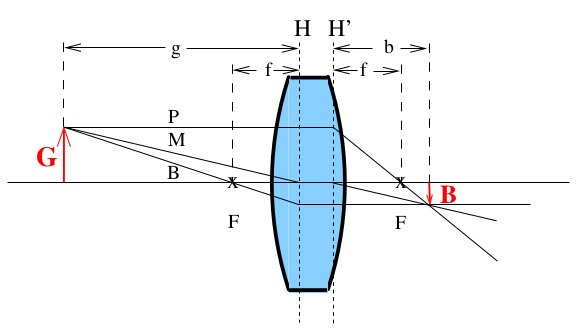
\includegraphics[height=5cm]{plots/Linse3.png}
        \caption{Eine dicke konvexe Linse\cite{Versuchsanleitung}.}
        \label{fig:konvex_dick}
    \end{subfigure}
    \begin{subfigure}{0.48\textwidth}
        \centering
        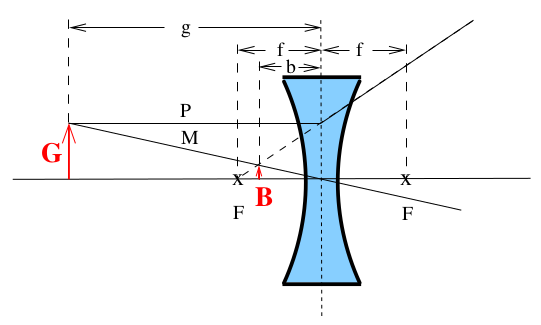
\includegraphics[height=5cm]{plots/Linse2.png}
        \caption{Eine konkave Linse\cite{Versuchsanleitung}.}
        \label{fig:konkav}
    \end{subfigure}
    \caption{Eine dicke Sammellinse und eine Zerstreuungslinse.}
    \label{fig:konvex_konkav}
\end{figure}
Die Mittelebene kann hier nicht als Näherung für den Ort des Abknicken der Strahlen genommen werden, sondern es muss 
zwischen den zwei eingezeichneten Hauptebenen $H$ und $H'$ unterschieden werden. Wie in der Abbildung deutlich wird, 
müssen alle Strahlen in dem Bereich zwischen den beiden Hauptebenen parallel zur optischen Achse verlaufen, bevor oder nachdem 
sie brechen. 
Außerdem werden die Abstände bis zur jeweiligen Hauptebene und nicht zur Mitte der Linse gemessen. 

Da bei dünnen Linsen der Abstand zwischen den beiden Hauptebenen verschwindend gering ist, ist es in dem Fall eine gute Näherung, 
die Hauptebenen in der Mittelebene als vereint anzusehen.  

Die andere, hier interessante Linsenform ist die konkave Zerstreuungslinse. Sie verdankt ihren Namen dem Umstand, dass 
sie parallel einfallendes Licht in alle Richtungen streut, wie in Abbildung \ref{fig:konkav} zu sehen ist. 
Dass sich einfallende Strahlen wieder in einem Punkt treffen, ist also nicht auf der anderen Seite der Linse möglich, jedoch 
auf der Gegenstandsseite. Da die Größen $f$ und $b$ für die Seite hinter der Linse als positiv angenommen werden, 
wie es bei den Sammellinsen der Fall ist, sind sie für Zerstreuungslinsen negativ definiert. 

Da das Bild einer Zerstreuungslinse auf der gleichen Seite wie der des Gegenstands entsteht, bekommt es die Bezeichnung 
\textit{virtuelles Bild}, im Gegensatz zum \textit{reellen Bild} einer Sammellinse\cite{Versuchsanleitung}. 

Es gibt zwei Gleichungen, die die Geometrie der Strahlengänge zusammenfassen; zum einen wäre da das Abbildungsgesetz 
\begin{equation}
    V=\frac{B}{G}=\frac{b}{g}\,,
    \label{eqn:Abbildungsgesetz}
\end{equation}
in dem $V$ der sogenannte Abbildungsmaßstab ist, sowie die Linsengleichung 
\begin{equation}
    \frac{1}{f}=\frac{1}{b}+\frac{1}{g}\,,
    \label{eqn:Linsengleichung}
\end{equation}
die Aussagen über die linsenspezifische Brennweite $f$ zulässt. 
Unbedingt zu beachten hierbei ist, dass bei dicken Linsen die Abstände nicht bis zur Mittelebene, sondern bis zur jeweiligen 
Hauptebene aufgenommen werden. Nur so verliert die Linsengleichung nicht ihre Gültigkeit\cite{Versuchsanleitung}. 

Eine weitere wichtige Größe ist die Brechkraft $D:=\sfrac{1}{f}$, die in der Einheit $\si{\per\meter}=\mathrm{dpt}$ angegeben wird. 
Werden mehrere Linsen hintereinander positioniert, können ihre Brechkräfte addiert werden, um diese modellierend zu einer 
gesamten Linse zusammenzufassen\cite{Versuchsanleitung}: 
\begin{equation*}
    D=\sum_i D_i = \sum_i \frac{1}{f_i}=\frac{1}{f}\,.
\end{equation*}

Eine weitere Näherung ist, dass im Prinzip der optischen Achse fernere Strahlen stärker von der Linse gebrochen werden, als 
solche, die nahe der optischen Achse verlaufen. Dies wird sphärischen Abberation genannt. 
Dadurch wird das Bild im Allgemeinen unscharf, da der Brennpunkt der achsenfernen Strahlen sich näher bei der Linse befindet. 
Die Unschärfe kann vermieden werden, indem mit einer Irisblende oder auf anderen Wegen die äußeren Strahlen ausgeblendet werden. 

Eine weiterer Linsenfehler ist die sogenannte chromatische Abberation. 
Diese beschreibt das unterschiedliche Brechungsverhalten von Licht mit verschiedener Wellenlänge, was der wellenlängenabhängigen Dispersion geschuldet ist. 
Rotes Licht mit einer größeren Wellenlänge wird dabei weniger stark gebrochen als blaues Licht, welches eine geringere Wellenlänge besitzt. 
Dadurch verschiebt sich der Brennpunkt blauen Lichts näher zur Linse hin und der von rotem Licht entfernt sich\cite{Versuchsanleitung}. 

\subsection{Methode von Bessel}

Ziel der Methode ist die Bestimmung der unbekannten Brennweite einer Linse. 
Demnach wird der Abstand zwischen Gegenstand und Bild (meist ein Schirm, auf dem die Lichtstrahlen sichtbar 
gemacht werden) konstant gehalten und eine Linse in dem Zwischenraum verschoben. 
Der Abstand $e=g+b$ verändert sich also nicht. 
Es werden zwei verschiedene Positionen der Linsen durch Verschieben gesucht, bei denen das Bild auf dem Schirm scharf wird. 
Aufgrund der Symmetrie ergibt sich, dass $b_1=g_2$ und $b_2=g_1$ gilt. 
Im Allgemeinen kann festgestellt werden, dass bei $g<b$ das Bild den Gegenstand vergrößert abbildet, bei $g>b$ genau anders herum. 
Dies wird in Abbildung \ref{fig:Bessel} unter anderem veranschaulicht. 

\begin{figure}
    \centering
    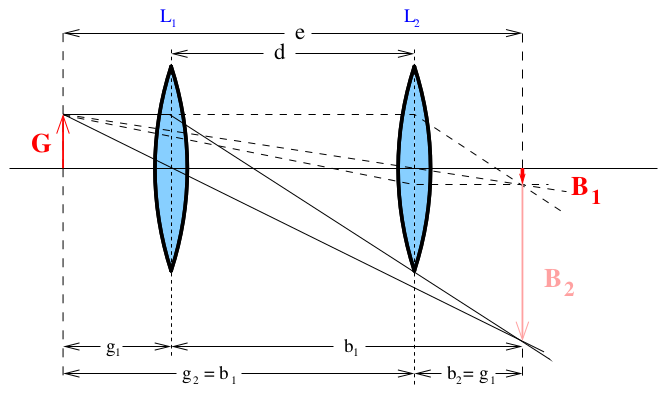
\includegraphics[width=0.75\textwidth]{plots/2Linsen.png}
    \caption{Die schematische Versuchsanordnung bei der Methode von Bessel\cite{Versuchsanleitung}.}
    \label{fig:Bessel}
\end{figure}

Dem entsprechend bleibt die Differenz zum Betrag $d=|g-b|$ ebenfalls unverändert. 
Setzt man die Ausdrücke in die Linsengleichung \eqref{eqn:Linsengleichung} ein, erhält man den Ausdruck\cite{Versuchsanleitung} 
\begin{equation}
    f=\frac{e^2-d^2}{4e}\,.
    \label{eqn:Bessel}
\end{equation}

\subsection{Methode von Abbe}

Mit der Methode von Abbe kann zusätzlich zu der Brennweite die Lage der Hauptebenen zweier Linsen bestimmt werden. 
Hierzu wird Abbildung \ref{fig:Abbe} betrachtet. 
\begin{figure}
    \centering
    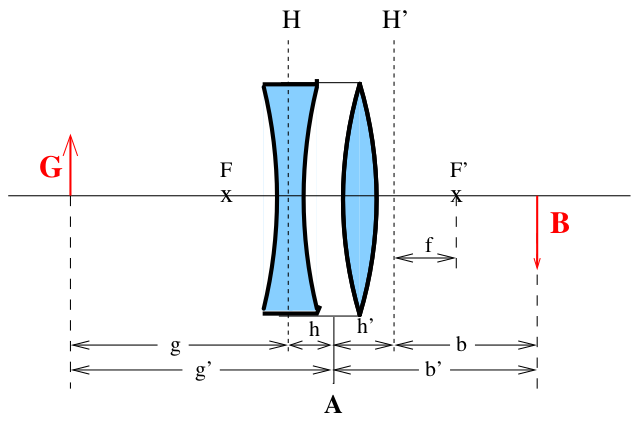
\includegraphics[width=0.75\textwidth]{plots/2LinsenTeil2.png}
    \caption{Strahlengangkonstruktion bei der Methode von Abbe\cite{Versuchsanleitung}.}
    \label{fig:Abbe}
\end{figure}
Da die genaue Lage der Hauptebenen unbekannt ist, wird ein bezüglich der Linsen fester Punkt $A$ gewählt, zu dem die Abstände $g'$ und $b'$ gemessen werden. 
Dementsprechend darf die Lage der Linsen zueinander während der Messung ebenfalls nicht verändert werden.
Es werden je Linsenposition die Werte für den Abbildungsmaßstab $V$ und für die Abstände $g'$ und $b'$ aufgenommen. 
Mithilfe der Linsengleichung \eqref{eqn:Linsengleichung} und dem Abbildungsgesetz \eqref{eqn:Abbildungsgesetz} ergeben sich die Zusammenhänge 
\begin{align}
    g'&=g+h &=f\cdot (1+\frac{1}{V})+h \qquad \text{und}\\
    b'&=b+h'&=f\cdot (1+V)+h'
\end{align}
Mithilfe zweier linearer Regressionen zu den Wertepaaren $(1+\sfrac{1}{V},g')$ und $(1+V,b')$ lassen sich aus den Geradenparametern 
die Größen $h$, $h'$ und $f$ bestimmen\cite{Versuchsanleitung}. 